\clearpage
\subsection{premi/client/trailsEditor}
\begin{figure}[h]
\begin{center}
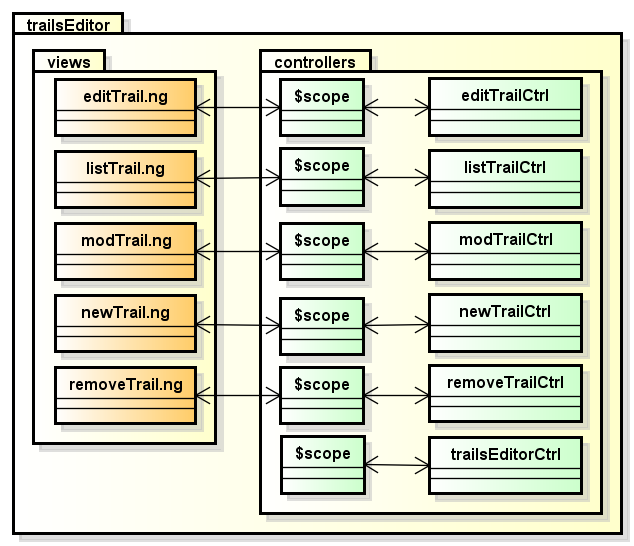
\includegraphics[scale=0.55]{img/diapkg/trailsEditor.png}
\caption{Diagramma del package premi/client/trailsEditor}
\end{center}
\end{figure}

%-------  diagramma di un template %
\subsubsection{premi/client/trailsEditor/views/basicToolbar.ng}

\begin{description}
%-------  descrizione del template%
\item[Descrizione] \hfill \\
	Template della vista associata allo \textit{\$scope} di \textit{basicToolbarCtrl}. Fornisce una toolbar per la navigazione tra le varie fasi della modifica della presentazione
\item[Note] \hfill \\
	\begin{itemize}
			\item Deve possedere un bottone per ogni fase dell'editor (Gestione Frame, Gestione Infografica e Gestione Trail)
			\item Deve possedere un bottone per l'uscita dall'editor
	\end{itemize}
\end{description}

%-------  diagramma di un template %
\subsubsection{premi/client/trailsEditor/views/editTrail.ng}

\begin{description}
%-------  descrizione del template%
\item[Descrizione] \hfill \\
	Template della vista associata allo \textit{\$scope} di \textit{editTrailCtrl}. Permette la modifica del titolo del trail selezionato dall'utente
\item[Note] \hfill \\
	\begin{itemize}
			\item Mostra il titolo del trail in un input HTML$_G$, modificabile, attraverso l'attributo dello scope \textit{Trail.title}
			\item Possiede un bottone associato al metodo \textit{save()} dello \textit{\$scope} per salvare le modifiche apportate al Trail
			\item Possiede un bottone associato al metodo \textit{discard()} dello \textit{\$scope} per annullare le modifiche effettuate sul trail
	\end{itemize}
\end{description}


%-------  diagramma di un template %
\subsubsection{premi/client/trailsEditor/views/listTrail.ng}

\begin{description}
%-------  descrizione del template%
\item[Descrizione] \hfill \\
	Template della vista associata allo \textit{\$scope} di \textit{listTrailCtrl}. Mostra la lista dei percorsi creati finora dall'utente associati alla presentazione
\item[Note] \hfill \\
	\begin{itemize}
			\item mostra una lista di tutti i percorsi attraverso l'attributo dello scope \textit{Trails}
			\item mostra una lista di tutti i frame inseribili attraverso il metodo dello scope \textit{getFramesId()}
	\end{itemize}
\end{description}

%-------  diagramma di un template %
\subsubsection{premi/client/trailsEditor/views/modTrail.ng}

\begin{description}
%-------  descrizione del template%
\item[Descrizione] \hfill \\
	Template della vista associata allo \textit{\$scope} di \textit{modTrailCtrl}. Deve consentire la modifica di un percorso in tutti i suoi attributi:
	\begin{itemize}
			\item inserimento di un frame in qualsiasi punto del percorso
			\item inserimento dello stesso frame più volte nel percorso
						\item spostamento di un frame da un punto all'altro del percorso
			\item eliminazione di un frame dal percorso
			\item trasformazione del frame in checkpoint
			\item elimiazione di un checkpoint
	\end{itemize}
\end{description}

%-------  diagramma di un template %
\subsubsection{premi/client/trailsEditor/views/newTrail.ng}

\begin{description}
%-------  descrizione del template%
\item[Descrizione] \hfill \\
	Template della vista associata allo \textit{\$scope} di \textit{newTrailCtrl}. Fornisce all'utente i comandi per l'inserimento di un novo trail associato alla presentazione nel database
\item[Note] \hfill \\
	\begin{itemize}
			\item Mostra un input HTML$_G$ associato all'attributo dello scope \textit{title} per l'inserimento del titolo del trail
			\item Possiede un bottone associato al metodo \textit{save()} dello \textit{\$scope} per salvare il nuovo Trail nel database
			\item Possiede un bottone associato al metodo \textit{discard()} dello \textit{\$scope} per annullare il processo di creazione del trail
	\end{itemize}
\end{description}

%-------  diagramma di un template %
\subsubsection{premi/client/trailsEditor/views/removeTrail.ng}

\begin{description}
%-------  descrizione del template%
\item[Descrizione] \hfill \\
	Template della vista associata allo \textit{\$scope} di \textit{removeTrailCtrl}. Fornisce all'utente i comandi per la rimozione di un trail associato alla presentazione dal database
\item[Note] \hfill \\
	\begin{itemize}
			\item Mostra un messaggio di conferma eliminazione del trail
			\item Possiede un bottone associato al metodo \textit{remove()} dello \textit{\$scope} confermare la rimozione
			\item Possiede un bottone associato al metodo \textit{discard()} dello \textit{\$scope} per annullare il processo di rimozione del trail
	\end{itemize}
\end{description}

































%-------  diagramma della classe%
\subsubsection{premi/client/trailsEditor/controllers/basicToolbarCtrl}
\begin{figure}[h]
\begin{center}
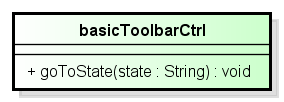
\includegraphics[scale=0.55]{img/diacla/basicToolbarCtrl.png}
\caption{Diagramma della classe premi/client/trailsEditor/controllers/basicToolbarCtrl}
\end{center}
\end{figure}


\begin{description}
%-------  descrizione della classe%
\item[Descrizione] \hfill \\
	Controller della view \textit{basicToolbar.ng}. Fornisce, tramite lo \textit{\$scope} un metodo per passaggio da un editor all'altro
	
%-------  lista dei metodi%	
\item[Metodi] \hfill \\

	% -- inizio metodo -- %
	\begin{description}
		\item[\textbf{\color{blue}+ goToState(state : String) : void			}] \hfill \\
			Tramite il metodo \textit{\$state.go} cambia "stato" dell'editor, passando da una fase di creazione della presentazione all'altra.
			
		\begin{description}
			% -- lista argomenti del metodo -- %
			\item[Argomenti] \hfill \\
				\begin{itemize}
				
					\item \textbf{state : String			} \hfill \\
					Il nuovo stato dell'editor. Gli stati dell'editor al momento sono:
					\begin{itemize}
						\item "premi.editor.frame"
						\item "premi.editor.infographic"
						\item "premi.editor.trails"
					\end{itemize}
					
				\end{itemize}
		\end{description}
	\end{description}
	% -- fine metodo -- %	
		
\end{description}



%-------  diagramma della classe%
\subsubsection{premi/client/trailsEditor/controllers/editTrailCtrl}
\begin{figure}[h]
\begin{center}
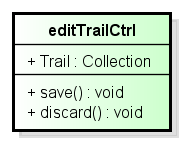
\includegraphics[scale=0.55]{img/diacla/editTrailCtrl.png}
\caption{Diagramma della classe premi/client/trailsEditor/controllers/editTrailCtrl}
\end{center}
\end{figure}


\begin{description}
%-------  descrizione della classe%
\item[Descrizione] \hfill \\
	Controller della view \textit{editTrail.ng}. Fornisce, tramite lo \textit{\$scope}, metodi e attributi necessari alla modifica del titolo di un trail
	
	
%-------  lista delle classi associate%	
\item[Dipendenze] \hfill \\
	\begin{itemize}
		\item \textbf{client/presentation/lib/databaseAPI}: per salvare il trail modificato
	\end{itemize}
	
	
%-------  lista degli Attributi%	
\item[Attributi] \hfill \\
	\begin{description}
		\item[\textbf{- Trail:Collection			}] \hfill \\
			Collezione di MongoDB degli attributi di un trail
	\end{description}
	
%-------  lista dei metodi%	
\item[Metodi] \hfill \\

	% -- inizio metodo -- %
	\begin{description}
		\item[\textbf{\color{blue}+ save() : void			}] \hfill \\
			Utilizza il metodo \textit{+ updateTrailTitle(idTrail, title)} di databaseAPI per l'aggiornamento del Trail nel database. Aggiorna poi la pagina con il cambiamento apportato
	\end{description}
	% -- fine metodo -- %		
	
	% -- inizio metodo -- %
	\begin{description}
		\item[\textbf{\color{blue}+ discard() : void			}] \hfill \\
			Annulla le modifiche effettuate dall'utente sul titolo del trail. Aggiorna poi la pagina riportandola allo stato precedente alla modifica
	\end{description}
	% -- fine metodo -- %		

	
\end{description}



%-------  diagramma della classe%
\subsubsection{premi/client/trailsEditor/controllers/listTrailCtrl}
\begin{figure}[h]
\begin{center}
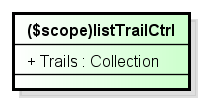
\includegraphics[scale=0.55]{img/diacla/listTrailCtrl.png}
\caption{Diagramma della classe premi/client/trailsEditor/controllers/listTrailCtrl}
\end{center}
\end{figure}


\begin{description}
%-------  descrizione della classe%
\item[Descrizione] \hfill \\
	Controller della view \textit{listTrail.ng}. Fornisce, tramite lo \textit{\$scope}, la lista dei trails associati alla presentazione che l'utente sta modificando
	
	
%-------  lista degli Attributi%	
\item[Attributi] \hfill \\
	\begin{description}
		\item[\textbf{- Trails:Collection			}] \hfill \\
			Collezione di MongoDB di tutti i trails associati alla presentazione (vengono pubblicati dal pattern publish-subscribe$_G$ al caricamento della pagina)	
	\end{description}
\end{description}








%-------  diagramma della classe%
\subsubsection{premi/client/trailsEditor/controllers/modTrailCtrl}
\begin{figure}[h]
\begin{center}
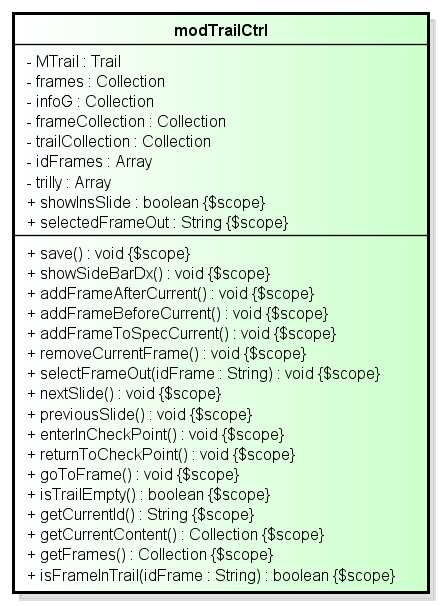
\includegraphics[scale=0.55]{img/diacla/modTrailCtrl.png}
\caption{Diagramma della classe premi/client/trailsEditor/controllers/modTrailCtrl}
\end{center}
\end{figure}


\begin{description}
%-------  descrizione della classe%
\item[Descrizione] \hfill \\
	Controller della view \textit{modTrail.ng}. Permette, tramite lo \textit{\$scope}, di modificare un trail in ogni suo aspetto, aggiungendo o togliendo frame, o creando percorsi di specializzazione. Fornisce all'utente la possibilità di scorrere il percorso con i quattro tasti "freccia" della tastiera
	
	
%-------  lista delle classi associate%	
\item[Dipendenze] \hfill \\
	\begin{itemize}
		\item \textbf{premi/client/presentation/Trail}: per la gestione del trail
	\end{itemize}
	
	
%-------  lista degli Attributi%	
\item[Attributi] \hfill \\
	\begin{description}
		\item[\textbf{- MTrail : Trail			}] \hfill \\
			Oggetto Trail da modificare. Inizialmente vuoto, dev'essere inizializzato con gli attributi di trailCollection
		\item[\textbf{- frames : Collection			}] \hfill \\
			Collezione di frames, nella forma \textit{id\_frame} : frame\_data
		\item[\textbf{- infoG : Collection			}] \hfill \\
			Collezione degli attributi dell'infografica della presentazione
		\item[\textbf{- frameCollection : Collection			}] \hfill \\
			Collezione di MongoDB$_G$ di tutti i frames della presentazione che sono stati inseriti nell'infografica
		\item[\textbf{- trailCollection : Collection			}] \hfill \\
			Collezione di MongoDB$_G$ di attributi del trail da modificare.
		\item[\textbf{- idFrames : Array			}] \hfill \\
			Array di codici identificativi dei frames presenti in FrameCollection
		\item[\textbf{- trilly : Array			}] \hfill \\
			Matrice vuota, utilizzata come variabile d'appoggio per l'utilizzo del metodo di MTrail initPath per la sua inizializzazione
		\item[\textbf{+ showInSide : boolean			}] \hfill \\
			Indica se la barra di destra dell'editor dev'essere visualizzata (\textit{true}) o meno (\textit{false})
		\item[\textbf{+ selectedFrameOut : String			}] \hfill \\
			È il frame che l'utente sta selezionando nella lista di tutti i frame della presentazione
	\end{description}
	
	
%-------  lista dei metodi%	
\item[Metodi] \hfill \\

	% -- inizio metodo -- %
	\begin{description}
		\item[\textbf{\color{blue}+ save() : void			}] \hfill \\
			utilizza il metodo updateTrail di \$meteor per il salvataggio della slide
	\end{description}
	% -- fine metodo -- %	
	
	% -- inizio metodo -- %
	\begin{description}
		\item[\textbf{\color{blue}+ showSideBarDx() : void			}] \hfill \\
			Attiva o disattiva la barra laterale destra dell'editor impostando a \textit{true} showInSide se era impostato a \textit{false} e viceversa
	\end{description}
	% -- fine metodo -- %	
	
	% -- inizio metodo -- %
	\begin{description}
		\item[\textbf{\color{blue}+ addFrameAfterCurrent()			}] \hfill \\
			utilizza il metodo insertSlideAfterCurrent di MTrail inserire la slide attualmente selezionata(selectedFrameOut) nella lista dopo quella selezionata nel percorso
	\end{description}
	% -- fine metodo -- %	
	
	% -- inizio metodo -- %
	\begin{description}
		\item[\textbf{\color{blue}+ addFrameAfterCurrent()			}] \hfill \\
			utilizza il metodo insertSlideAfterCurrent di MTrail per inserire la slide attualmente selezionata(selectedFrameOut) nella lista prima di quella selezionata nel percorso
	\end{description}
	% -- fine metodo -- %		
	
	% -- inizio metodo -- %
	\begin{description}
		\item[\textbf{\color{blue}+ addFrameBeforeCurrent()			}] \hfill \\
			utilizza il metodo insertSlideBeforeCurrent di MTrail per inserire la slide attualmente selezionata(selectedFrameOut) nella lista prima di quella selezionata nel percorso
	\end{description}
	% -- fine metodo -- %	
	
	% -- inizio metodo -- %
	\begin{description}
		\item[\textbf{\color{blue}+ addFrameToSpecCurrent()			}] \hfill \\
			utilizza il metodo insertSlideInSpecTrail di MTrail per inserire la slide attualmente selezionata(selectedFrameOut) nella lista nel percorso di specializzazione di quella selezionata nel percorso
	\end{description}
	% -- fine metodo -- %	
	
	% -- inizio metodo -- %
	\begin{description}
		\item[\textbf{\color{blue}+ removeCurrentFrame()			}] \hfill \\
			utilizza il metodo removeCurrentSlide di MTrail per rimuovere la slide selezionata nel percorso
	\end{description}
	% -- fine metodo -- %	
	
	% -- inizio metodo -- %
	\begin{description}
		\item[\textbf{\color{blue}+ selectFrameOut(idFrame : String) : void			}] \hfill \\
			Copia il codice identificativo del frame ricevuto dentro selectedFrameOut, rendendolo in questo modo selezionato.
			
		\begin{description}
			% -- lista argomenti del metodo -- %
			\item[Argomenti] \hfill \\
				\begin{itemize}
				
					\item \textbf{idFrame : String			} \hfill \\
					Il codice identificativo del frame da selezionare
					
				\end{itemize}
			
		\end{description}
	\end{description}
	% -- fine metodo -- %	
	
	% -- inizio metodo -- %
	\begin{description}
		\item[\textbf{\color{blue}+ nextSlide()			}] \hfill \\
			utilizza il metodo nextSlide di MTrail per avanzare di un passo nel trail
	\end{description}
	% -- fine metodo -- %	
	
	% -- inizio metodo -- %
	\begin{description}
		\item[\textbf{\color{blue}+ previousSlide()			}] \hfill \\
			utilizza il metodo nextSlide di MTrail per retrocedere di un passo nel trail
	\end{description}
	% -- fine metodo -- %	
	
	% -- inizio metodo -- %
	\begin{description}
		\item[\textbf{\color{blue}+ enterInCheckPoint()			}] \hfill \\
			utilizza il metodo enterInCheckPoint di MTrail per entrare nel percorso di specializzazione associato al frame attualmente selezionato nel percorso, se il frame funge da checkpoint
	\end{description}
	% -- fine metodo -- %	
	
	% -- inizio metodo -- %
	\begin{description}
		\item[\textbf{\color{blue}+ returnToCheckPoint()			}] \hfill \\
			utilizza il metodo returnToCheckPoint di MTrail per uscire dal percorso di specializzazione e tornare al percorso dove risiede il checkpoint
	\end{description}
	% -- fine metodo -- %	
	
	% -- inizio metodo -- %
	\begin{description}
		\item[\textbf{\color{blue}+ goToFrame(idSlide : String) : void			}] \hfill \\
			Rende un frame selezionato nel percorso
			
		\begin{description}
			% -- lista argomenti del metodo -- %
			\item[Argomenti] \hfill \\
				\begin{itemize}
				
					\item \textbf{idSlide : String			} \hfill \\
					Il codice identificativo del frame da selezionare
					
				\end{itemize}
			
		\end{description}
	\end{description}
	% -- fine metodo -- %
	
	
	% -- inizio metodo -- %
	\begin{description}
		\item[\textbf{\color{blue}+ isTrailEmpty() : bool		}] \hfill \\
			utilizza il metodo isTrailEmpty di MTrail per restituire \textit{true} se il percorso è vuoto, \textit{false} altrimenti
	\end{description}
	% -- fine metodo -- %	
	
	% -- inizio metodo -- %
	\begin{description}
		\item[\textbf{\color{blue}+ getCurrentId() : String		}] \hfill \\
			utilizza il metodo getCurrentId di MTrail per restituire il codice identificativo del frame attualmente selezionato nel percorso
	\end{description}
	% -- fine metodo -- %		
	
	% -- inizio metodo -- %
	\begin{description}
		\item[\textbf{\color{blue}+ getCurrentContent() : Collection		}] \hfill \\
			utilizza il metodo getCurrentId di MTrail per ricevere il codice identificativo del frame attualmente selezionato nel percorso, per poi utilizzarlo per restituire gli attributi del frame, reperibili dalla collezione frames
	\end{description}
	% -- fine metodo -- %
	
	% -- inizio metodo -- %
	\begin{description}
		\item[\textbf{\color{blue}+ getFrames() : Collection		}] \hfill \\
			restituisce l'intera collezione frames
	\end{description}
	% -- fine metodo -- %	
	
	
	% -- inizio metodo -- %
	\begin{description}
		\item[\textbf{\color{blue}+ isFrameInTrail(idFrame : String) : bool			}] \hfill \\
			utilizza il metodo isSlideInTrail di MTrail per restituire \textit{true} se il frame è nel percorso, \textit{false} altrimenti
			
		\begin{description}
			% -- lista argomenti del metodo -- %
			\item[Argomenti] \hfill \\
				\begin{itemize}
				
					\item \textbf{idFrame : String			} \hfill \\
					Il codice identificativo del frame da cercare
					
				\end{itemize}
			
		\end{description}
	\end{description}
	% -- fine metodo -- %	
	
\end{description}	
	
	
	
	
	
	
	
	
	
	
	%-------  diagramma della classe%
\subsubsection{premi/client/trailsEditor/controllers/newTrailCtrl}
\begin{figure}[h]
\begin{center}
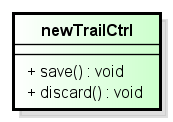
\includegraphics[scale=0.55]{img/diacla/newTrailCtrl.png}
\caption{Diagramma della classe premi/client/trailsEditor/controllers/newTrailCtrl}
\end{center}
\end{figure}


\begin{description}
%-------  descrizione della classe%
\item[Descrizione] \hfill \\
	Controller della view \textit{newTrail.ng}. Fornisce, tramite lo \textit{\$scope}, metodi e attributi necessari alla creazione di un nuovo trail
	
	
%-------  lista delle classi associate%	
\item[Dipendenze] \hfill \\
	\begin{itemize}
		\item \textbf{premi/client/presentation/lib/databaseAPI}: per i metodi necessari al salvataggio del nuovo trail nel database
	\end{itemize}
	
	
%-------  lista dei metodi%	
\item[Metodi] \hfill \\

	% -- inizio metodo -- %
	\begin{description}
		\item[\textbf{\color{blue}+ save() : void			}] \hfill \\
			Utilizza il metodo \textit{+ insertTrail} di databaseAPI per il salvataggio del nuovo Trail nel database. Aggiorna poi la pagina con il cambiamento apportato al database
	\end{description}
	% -- fine metodo -- %		
	
	% -- inizio metodo -- %
	\begin{description}
		\item[\textbf{\color{blue}+ discard() : void			}] \hfill \\
			Annulla il processo di creazione del trail. Aggiorna poi la pagina riportandola allo stato precedente
	\end{description}
	% -- fine metodo -- %	

\end{description}
	






	%-------  diagramma della classe%
\subsubsection{premi/client/trailsEditor/controllers/removeTrailCtrl}
\begin{figure}[h]
\begin{center}
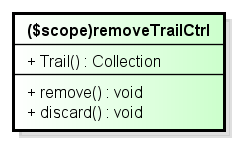
\includegraphics[scale=0.55]{img/diacla/removeTrailCtrl.png}
\caption{Diagramma della classe premi/client/trailsEditor/controllers/removeTrailCtrl}
\end{center}
\end{figure}


\begin{description}
%-------  descrizione della classe%
\item[Descrizione] \hfill \\
	Controller della view \textit{removeTrail.ng}. Fornisce, tramite lo \textit{\$scope}, metodi e attributi necessari all'eliminazione di un trail
	
	
%-------  lista delle classi associate%	
\item[Dipendenze] \hfill \\
	\begin{itemize}
		\item \textbf{premi/client/presentation/lib/databaseAPI}: per i metodi necessari all'eliminazione del trail dal database
	\end{itemize}
	
	
%-------  lista dei metodi%	
\item[Metodi] \hfill \\

	% -- inizio metodo -- %
	\begin{description}
		\item[\textbf{\color{blue}+ remove() : void			}] \hfill \\
			Utilizza il metodo \textit{+ removeTrail} di databaseAPI per la rimozione del trail dal database. Aggiorna poi la pagina con il cambiamento apportato al database
	\end{description}
	% -- fine metodo -- %		
	
	% -- inizio metodo -- %
	\begin{description}
		\item[\textbf{\color{blue}+ discard() : void			}] \hfill \\
			Annulla il processo di eliminazione del trail. Aggiorna poi la pagina riportandola allo stato precedente
	\end{description}
	% -- fine metodo -- %	

\end{description}
	







%-------  diagramma della classe%
\subsubsection{premi/client/trailsEditor/controllers/trailsEditorCtrl}
\begin{figure}[h]
\begin{center}
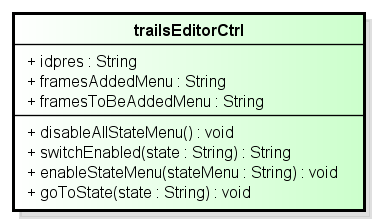
\includegraphics[scale=0.55]{img/diacla/trailsEditorCtrl.png}
\caption{Diagramma della classe premi/client/trailsEditor/controllers/trailsEditorCtrl}
\end{center}
\end{figure}


\begin{description}
%-------  descrizione della classe%
\item[Descrizione] \hfill \\
	Controller generale dell'editor dei trail. Prepara lo \textit{\$scope} con attributi e metodi utili alle viste e ai controller interni a questo editor.
	
	
%-------  lista degli Attributi%	
\item[Attributi] \hfill \\
	\begin{description}
		\item[\textbf{+ idPres : String			}] \hfill \\
			Codice identificativo della presentazione che l'utente sta modificando, è prelevato da \textit{\$stateParams}
		\item[\textbf{+ framesAddedMenu	: String		}] \hfill \\
			Indica se il menu dei frames aggiunti finora al trail è visualizzato (\textit{enabled}) o meno (\textit{disabled}
		\item[\textbf{+ framesToBeAddedMenu	: String		}] \hfill \\
			Indica se il menu di tutti i frames della presentazione è visualizzato (\textit{enabled}) o meno (\textit{disabled}
	\end{description}
	
	
%-------  lista dei metodi%	
\item[Metodi] \hfill \\

	% -- inizio metodo -- %
	\begin{description}
		\item[\textbf{\color{blue}+ disableAllStateMenu() : void			}] \hfill \\
			Disabilita i menu dei frame e aggiorna la pagina

	\end{description}
	% -- fine metodo -- %	
	
	% -- inizio metodo -- %
	\begin{description}
		\item[\textbf{\color{blue}+ switchEnabled(state : String) : void			}] \hfill \\
			Se lo stato ricevuto è '\textit{enabled}' lo rende '\textit{disabled}', e viceversa
			
		\begin{description}
			% -- lista argomenti del metodo -- %
			\item[Argomenti] \hfill \\
				\begin{itemize}
				
					\item \textbf{state : String			} \hfill \\
					Lo stato da abilitare/disabilitare
					
				\end{itemize}
		\end{description}
	\end{description}
	% -- fine metodo -- %	
	
	% -- inizio metodo -- %
	\begin{description}
		\item[\textbf{\color{blue}+ enableStateMenu(stateMenu : String) : void			}] \hfill \\
			Abilita il menu rappresentato da stateMenu
			
		\begin{description}
			% -- lista argomenti del metodo -- %
			\item[Argomenti] \hfill \\
				\begin{itemize}
				
					\item \textbf{stateMenu : String			} \hfill \\
					Il menu da abilitare, può essere: 
					\begin{itemize}
						\item frameAddedMenu
						\item framesToBeAddedMenu
					\end{itemize}
					
				\end{itemize}
		\end{description}
	\end{description}
	% -- fine metodo -- %	
	
	% -- inizio metodo -- %
	\begin{description}
		\item[\textbf{\color{blue}+ goToState(state : String) : void			}] \hfill \\
			Rimanda l'utente alla vista rappresentata dallo stato ricevuto
			
		\begin{description}
			% -- lista argomenti del metodo -- %
			\item[Argomenti] \hfill \\
				\begin{itemize}
				
					\item \textbf{state : String			} \hfill \\
					Lo stato che rappresenta la vista da mostrare all'utente
					
				\end{itemize}
		\end{description}
	\end{description}
	% -- fine metodo -- %
	
			

\end{description}